\documentclass[10pt]{article}

% DO NOT EDIT THE LINES BETWEEN THE TWO LONG HORIZONTAL LINES

%---------------------------------------------------------------------------------------------------------

% Packages add extra functionality.
\usepackage{times,graphicx,epstopdf,fancyhdr,amsfonts,amsthm,amsmath,algorithm,xspace,hyperref}
\usepackage[left=1in,top=1in,right=1in,bottom=1in]{geometry}
\usepackage{sect sty}	%For centering section headings
\usepackage{enumerate}	%Allows more labeling options for enumerate environments 
\usepackage{epsfig}
\usepackage[space]{grffile}
\usepackage{algpseudocode}

% This will set LaTeX to look for figures in the same directory as the .tex file
\graphicspath{.} %The dot means current directory.

\pagestyle{fancy}

\lhead{\WilliamsID}
\chead{Problem Set \PSNumber \ --- Problem \ProblemNumber}
\rhead{\today}
\lfoot{CSci 256: Algorithm Design}
\cfoot{\thepage}
\rfoot{Spring 2018}

% Some commands for changing header and footer format
\renewcommand{\headrulewidth}{0.4pt}
\renewcommand{\headwidth}{\textwidth}
\renewcommand{\footrulewidth}{0.4pt}

% These let you use common environments
\newtheorem{claim}{Claim}
\newtheorem{definition}{Definition}
\newtheorem{theorem}{Theorem}
\newtheorem{lemma}{Lemma}
\newtheorem{observation}{Observation}
\newtheorem{question}{Question}

\setlength{\parindent}{0cm}
\usepackage{tikz}
\usepackage{enumitem}
%---------------------------------------------------------------------------------------------------------

% DON'T CHANGE ANYTHING ABOVE HERE

% Edit below as instructed
\newcommand{\WilliamsID}{W3026623}	% Put you Williams ID in the braces
\newcommand{\PSNumber}{5}			% Put the problem set # in the braces
\newcommand{\ProblemNumber}{1}		% Put the problem # in the braces
\newcommand{\ProblemHeader}{Problem \ProblemNumber}	% Don't change this

\begin{document}

\vspace{\baselineskip}	% Add some vertical space
\textbf{I collaborated with:} 


\vspace{\baselineskip}	% Add some vertical space
\textbf{Problem}

Answer Exercise 1 (page 312) in Chapter 6 of your text.  For part (c) include a justification of correctness and a time/space complexity analysis.\\
\textbf{Solution}\\
\begin{enumerate}[label=\Alph*]
	\item 

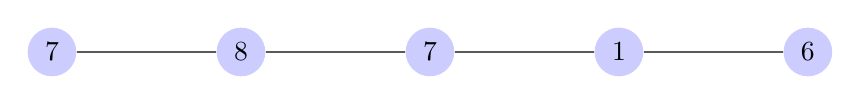
\begin{tikzpicture}
[scale=.8,auto=left,every node/.style={circle,fill=blue!20}]
\node (n6) at (1,8) {7};
\node (n4) at (4,8)  {8};
\node (n5) at (7,8)  {7};
\node (n1) at (10,8) {1};
\node (n2) at (13,8)  {6};

\foreach \from/\to in {n6/n4,n4/n5,n5/n1,n1/n2}
\draw (\from) -- (\to);

\end{tikzpicture}
\\The algorithm will return the set of nodes \{8,6\}, while the independent set of maximum total weigth is \{7,7,6\}.
\item 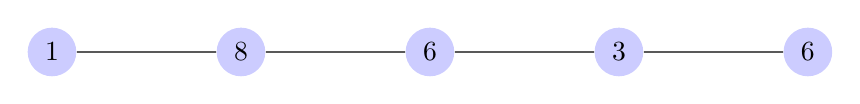
\begin{tikzpicture}
[scale=.8,auto=left,every node/.style={circle,fill=blue!20}]
\node (n6) at (1,8) {1};
\node (n4) at (4,8)  {8};
\node (n5) at (7,8)  {6};
\node (n1) at (10,8) {3};
\node (n2) at (13,8)  {6};

\foreach \from/\to in {n6/n4,n4/n5,n5/n1,n1/n2}
\draw (\from) -- (\to);

\end{tikzpicture}
\\The algorithm will return the set of nodes \{1,6,6\}, while the independent set of maximum total weigth is \{8,6\}.
\item The recurrence $opt(v_{i}) = \max (w_{i} + opt(v_{i-2}), opt(v_{i-1})$ tells us a dynamic programming approach for solving this problem. \\
\begin{algorithm*}[h] 
	\caption{returns an independent set of maximum total weight} 
	\begin{algorithmic}
		\State Start with $A$ equal to the empty array of size $n$
		\Function{opt}{$v$}
		\If {$v$ is adjacent to only one node of greater index or $v$ is the last node}
		\State $A[i] = w_{i}$ \State \Return $A[1]$
		\ElsIf {$A[i] > 0$}
		\State \Return $A[i]$
		\Else
		\State $A[i] = \max (w_{i} + opt(v_{i-2}), opt(v_{i-1}))$ \State \Return $A[i]$
		\EndIf
		\EndFunction
	\end{algorithmic}
\end{algorithm*}
\end{enumerate}

This algorithm builds the array of maximum total weights for independent sets for all nodes from $v_{1}$ to $v_{n}$. We can then just find the maximum entry of $A$ and trace subsequent maximum values of the remaining array to build up our answer. We will now prove why it works.
\begin{proof}
	Base Case: Let $g$ be a graph of only one node $v_{0}$. The independent set of maximum total weight is that only containing $v_{0}$. Our algorithm will see that $v_{0}$ is the last node of $g$ and will update $A[0] = w_{0}$. It will then return $\{v_{0}\}$ as it corresponds to the maximum weight.\\
	Inductive Hypothesis: Assume our algorithm works for all graphs that have up to $k$ nodes where $k \ge 1$.\\
	Inductive Step: We need to show our algorithm always returns an independent set of maximum total weight for a graph of $k+1$ nodes. Let $G$ be a graph of $k$ nodes labeled $v_{1}$ to $v_{k}$. If we add another node $v_{0}$ then we will need to see if $v_{0}$ is part of our independent set of maximum total weight. We will either include its weight to a maximum set of vertices not adjacent to $v_{0}$ (Note that this existing set corresponds to a graph of less than $k+1$ nodes and our inductive hypothesis assures the set is of maximum weights). Otherwise, we do not consider $w_{0}$ in our maximum set and we use the independent set of maximum total weight of $G$ (by our inductive hypothesis, the algorithm returns the proper set for $G$ as it has $k$ nodes).
\end{proof}
Time Complexity: $O(n)$ to build array + $O(n)$ to find set = $O(n)$\\
Space Complexity: Array of size $n\ O(n)$ + $n$ recursive calls for stack frame = $O(n)$
%End of feedback section

% DO NOT DELETE ANYTHING BELOW THIS LINE
\end{document}
